\notechapter{N-20230201}{Gravitational Field inside a Uniform Spherical Shell}

\section{Problem}

The note studies the classical shell theorem: the gravitational field produced by a uniform spherical shell at any interior point is zero.  The physical statement is simple, but the proof is a good training ground for geometric integration.

Let the shell have surface density \(\sigma\), center \(O\), and let \(P\) be an interior point.  We want to prove that the total gravitational field at \(P\) cancels.

\section{Geometric pairing method}

Choose the axis \(OP\).  A ray through \(P\) meets the sphere in two opposite small surface elements.  Although one element is farther away than the other, it also subtends a correspondingly larger area.  The inverse-square law and the area scaling cancel exactly.

\begin{figure}[H]
\centering
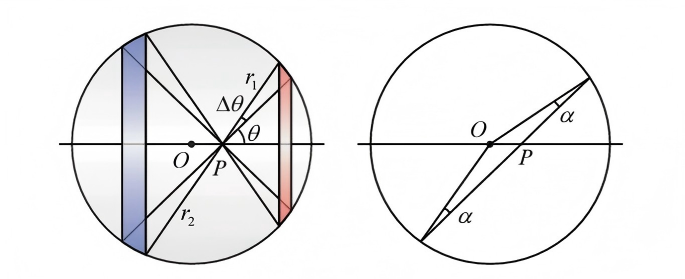
\includegraphics[width=.72\linewidth]{figures/N-20230201/01-shell-geometric-method.png}
\caption{Opposite surface elements seen from an interior point.}
\end{figure}

The note writes the masses of two corresponding small rings or patches as proportional to their areas.  If their distances from \(P\) are \(r_1,r_2\), then the gravitational magnitudes contain factors of the form
\[
  \frac{G\,dM_i}{r_i^2}.
\]
But \(dM_i\) itself is proportional to \(r_i^2\) times the same solid angle.  Therefore the two fields have equal magnitudes and opposite directions.  Pairing all such opposite elements gives total field zero.

This is the cleanest idea: the inverse-square law is exactly matched by the square scaling of area under fixed solid angle.

\section{Integral method}

The note also gives an integration method.  Let the field point be at distance \(r\) from the center.  A circular ring on the shell at polar angle \(\theta\) has mass
\[
  dM=2\pi R^2\sigma\sin\theta\,d\theta.
\]
The contribution along the axis is
\[
  dg=\frac{G\,dM}{\ell^2}\cos\alpha,
\]
where \(\ell\) is the distance from the ring to \(P\) and \(\alpha\) is the angle between the line of force and the axis.

\begin{figure}[H]
\centering
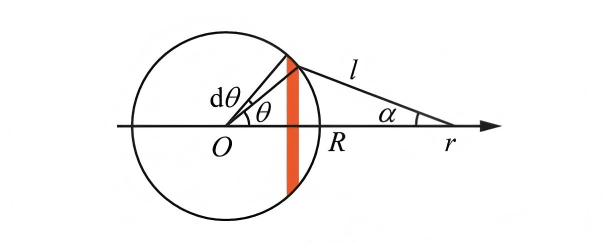
\includegraphics[width=.62\linewidth]{figures/N-20230201/02-shell-integral-method.png}
\caption{Ring integration for the field of a spherical shell.}
\end{figure}

Using the law of cosines and differentiating the relation between \(\ell\) and \(\theta\), the integral collapses to zero for \(r<R\).  The algebra is less transparent than the pairing proof, but it is more systematic and generalizes to other symmetric mass distributions.

\section{Connection with Newton's theorem}

The theorem has two parts:
\begin{enumerate}[(i)]
  \item outside a uniform spherical shell, the field is as if all mass were concentrated at the center;
  \item inside the shell, the field is zero.

\end{enumerate}
The note focuses on the second.  For a solid uniform ball, the interior field at radius \(r\) depends only on the mass inside radius \(r\), because outer spherical shells contribute zero.  Thus
\[
  g(r)=\frac{G M(r)}{r^2}\propto r
\]
inside a uniform solid sphere.


\section{Details of the solid-angle argument}

The pairing proof deserves more detail.  From the interior point \(P\), take a very small cone of solid angle \(d\Omega\).  It cuts two small patches from the spherical shell, one on the near side and one on the far side.  If their distances from \(P\) are \(r_1\) and \(r_2\), then the corresponding patch areas are, up to the same obliquity factor,
\[
  dS_i\propto r_i^2\,d\Omega .
\]
Their masses are \(dM_i=\sigma dS_i\).  The gravitational acceleration produced by each patch has magnitude
\[
  dg_i=G\frac{dM_i}{r_i^2}.
\]
The factor \(r_i^2\) in area cancels the inverse-square law.  The two patches lie in opposite directions along the same line through \(P\), so their vector contributions cancel.

This is the core reason the theorem is true.  It is not merely symmetry around the center of the sphere; the point \(P\) is not at the center.  The cancellation works because the inverse-square law exactly matches how apparent area scales with distance.

\section{Why the theorem would fail for a different force law}

If the force were proportional to \(1/r^3\) or \(1/r\), the same cancellation would not occur.  The near and far patches would still subtend the same solid angle, but their masses would scale like \(r^2\), while the force factor would scale differently.  Thus the shell theorem is a special consequence of the inverse-square law.

This also explains why the result is closely related to Gauss's law.  Inverse-square fields have constant flux through spheres.  A spherical shell contributes zero field inside because a Gaussian sphere inside the shell encloses no mass.

\section{Potential viewpoint}

Another way to understand the theorem is through gravitational potential.  The potential of a shell at an interior point is constant.  Since gravitational field is the negative gradient of potential,
\[
  \mathbf g=-\nabla V,
\]
a constant potential inside implies zero field.

This viewpoint is often cleaner in advanced mechanics: instead of adding vector forces directly, compute a scalar potential and then differentiate.  It also connects the shell theorem with harmonic functions and Laplace's equation.

\section{Expanded synthesis and advanced context}

The shell theorem is an early example of symmetry plus inverse-square law.  In modern language, it is closely related to Gauss's law: a spherically symmetric field has flux controlled by enclosed mass.  The geometric proof shows why the exponent \(2\) is special; the integral proof shows how symmetry reduces a surface integral to one variable.


\paragraph{Expanded synthesis.}
The common theme of this chapter is that an elementary limiting or computational rule becomes powerful only after one specifies the space in which the limiting process takes place. The earlier sections (`Problem`, `Geometric pairing method`, `Integral method`, `Connection with Newton's theorem`, `Details of the solid-angle argument`) may look like separate techniques, but they all ask the same question: which operations are stable under approximation? A derivative is stable first-order approximation,
\[
  f(a+h)=f(a)+L(h)+o(|h|),
\]
while an integral is stable accumulation with respect to a measure, and a convergent series is a limit in a chosen norm or topology.

The advanced bridge is functional-analytic. Uniform convergence is convergence in a sup norm; $L^p$ convergence is convergence in an integral norm; differentiability is the existence of a continuous linear approximation; many differential equations are operator equations $L[u]=f$. Theorems such as dominated convergence, the inverse function theorem, the projection theorem in Hilbert spaces, and semigroup existence results are refined answers to the same elementary concern: when may we pass from finite approximations to a genuine limiting object?

To use this viewpoint when rereading the original examples, identify the hidden stability condition. A Taylor expansion asks for control of the remainder. A change of variables asks for differentiability and Jacobian control. Termwise differentiation of a series asks for uniform convergence of derivative series. A differential-equation formula asks whether the operator is invertible under the imposed initial or boundary data. The elementary computation is the visible part; the advanced theory names the hypotheses that make it legitimate.
